\section{System Overview}
Human movement is a complex interplay between intentions within the brain and the physical environment. The though to 'walk-forward' triggers and array of intractable optimization  

In the following we will introduce a method for optimal synchronization between a Movement Model and a set of animations given Control Genomes. There are 4 main parts to the system. 
\begin{itemize}
    \item \textbf{Control Genomes} extracted from animations.
    \item \textbf{Movement Model} that generates a movement given Control Genomes.
    \item \textbf{Animation Aligment} and filtering. 
    \item \textbf{Optimization procedure} that fits exposed parameters of all the above systems to minimize the difference between the Movement Model- and animation trajectories.
\end{itemize}
Figure \ref{fig:movement:model} illustrates the definitions and concepts of a movement model.
\begin{figure}
    \centering
    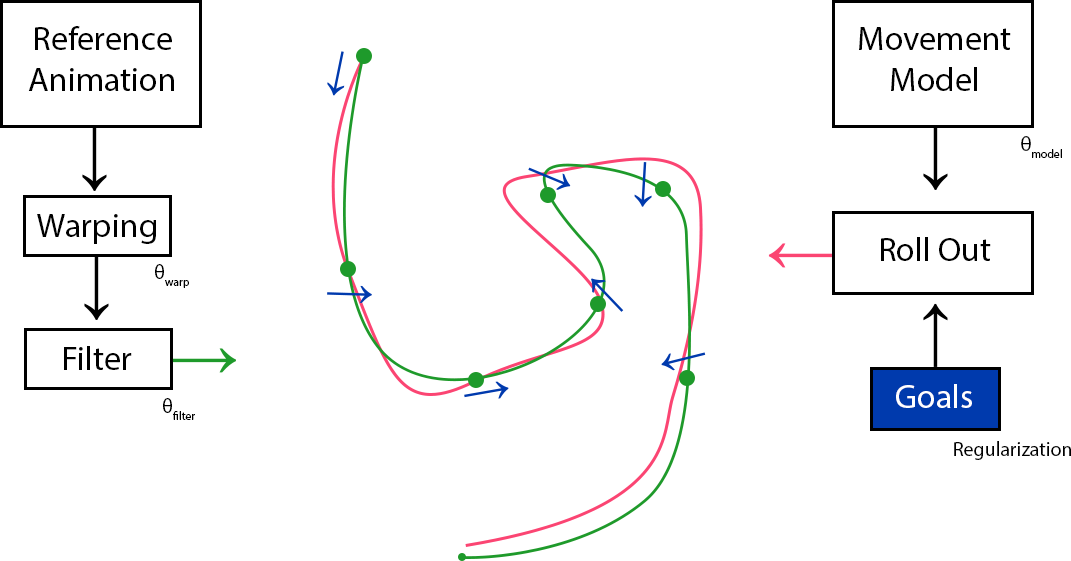
\includegraphics[width=0.75\columnwidth]{img/method-overview.png}
    \caption{Theta values indicate parameters subject to optimization. Goals are fixed to add regularization}.
    label{fig:movement:model}
\end{figure}

\section{Control Genomes}
We define Control Genomes as signals that can generate movement. They are a combination of intentions and enough contextual state to follow the Markov principle. As an example a position, direction and time is a Control Genome for a straight walk. Conversely a straight walk contains a latent Control Genome (position, direction, time). Under this naive framework we quickly realize that multiple straight walks could be associated with a single Control Genome. We further impose the constraint that Control Genomes must disambiguate movement, ie. a unique Control Genome maps to a unique movement. In our simple example we might resolve conflicts by adding a style parameter and assign values such as 'brisk walk' or 'dragging feet' to our Control Genomes. 

Control Genomes can have a direct counter part in the host application such as user input through a game controller or navigational path from an AI system, and therefore can also be viewed as tasks (ie. turn right) that are carried out by the animations. In general we want the Control Genomes to be of minimal size, since in the limit we could have the animation itself as the Control Genome. We say that a genome is in \textit{reduced} and \textit{segmented} form if it contains no repetitions and removal of information would break either the Markov property of the disambiguation constraint. 

\begin{figure}
    \centering
    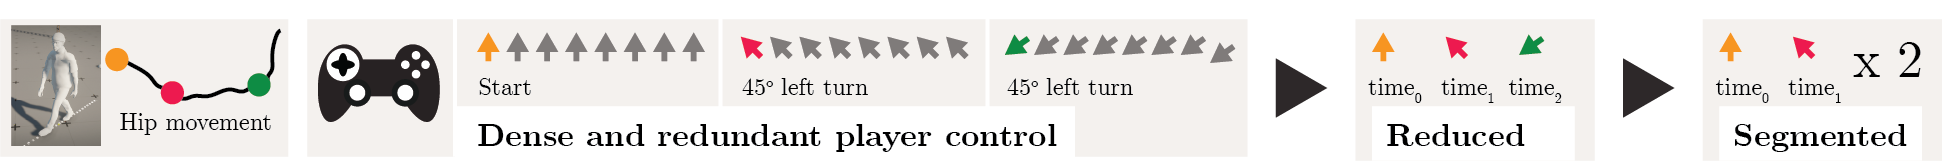
\includegraphics[width=1\columnwidth]{img/controlgenome.png}
    \caption{Control Genome}
    \label{fig:control:genome}
\end{figure}

Figure Fig. \ref{fig:control:genome} shows an example where an animation has been assigned a Control Genome. Each frame is annotated with a 2d-control direction corresponding to stick input from a game controller. A dense and redundant Control Genome contains the entire skeletal animation as well as the annotated directions. The animation has two similar right turns so we get a single segmented Control Genome by splitting the redundant genome in two identical parts. We then trim all unnecessary information from the genome to get the reduced form which only contain a starting position and two direction offset in time. This last step assumes that we are capable of regenerating the animation from the reduced genome using a procedure we will refer to as a \textit{Movement Model}. A [Control Genome, Movement Model]-pair describes an animation exactly when the Movement Model can regenerate the Animation from the Control Genome.  In practice it is not possible to develop accurate generative or predictive models for human movement. So we will allow our animations to undergo non destructive transformation such as smoothing and path adjustment, and only expect our model to regenerate a fraction of the complete signal, such as the trajectory. 

We will now proceed to a formalized description of Control Genomes.

The input to our system is an annotated animation. Let $\anim^{\dimas,\dimaa}_\dimat$ denote $\dimat$ frames of animation of a skeleton with $\dimas$ degrees of freedom, where each frame is given an $\dimaa$-dimensional annotation. We assume the presence of a Retrieve-and-Collapse procedure (automated or manual) that extracts all reduced and segmented Control Genomes present in the animation and for each maintains a pairing to all $k$ corresponding (un-annotated) segments of the source animation. With $i$ as the index and $\dimg$ as the dimensionality of the Control Genomes we have $\genome^g_i\in\reco(\anim^{\dimas,\dimaa}_\dimat)\rightarrow\anim^{\dimas,0}_{\dimae_0}\ldots\anim^{\dimas,0}_{\dimae_k}$ where $\dimae\ll\dimat$ refers to a segment of the full animation and $k$ is the number of segments matched to the $i$'th Control Genome.


We define two parametric projections to a shared $\dimes$-dimensional evaluation space as $\model(\paramm,\genome^{\dimg}) \rightarrow \mathcal{R}^{\dimes}$ and $\edit(\parame,\anim_{\dimae}^{\dimas,0}) \rightarrow \mathcal{R}^{\dimes}$. The evaluation space will usually have a natural counterpart in the application such as the trajectory (position and orientation of character over time).\\
Intuitively $\model$ is a Movement Model capable of generating movement (or more accurately an evaluation space representation) from the Control Genomes. $\edit$ corresponds to the adjustment we allow our animations to undergo, such a smoothing or more advanced manipulation. The optimal parameters for a single Control Genome are found as the minimization of the L2-norm.
\begin{subequations}
\begin{align}
    \gnorm(\paramm,\parame,\genome)&=\sum_{\anim_k\in\genome}{\frac{1}{2}|\model(\paramm,\genome)-\edit(\parame\anim_k)|^2}\label{eq:optim:single}\\
    \paramm^*,\parame^*&=\min_{\paramm,\parame}{\gnorm(\paramm,\parame,\genome)}
\end{align}
\end{subequations}
When we want constant parameters across the fitting of multiple Control Genomes $\genome_i\in\reco(\genome)$ an additional term is added to the minimization. 
\begin{equation}
    \vec{\paramm^*},\vec{\parame^*}=\min_{\paramm,\parame}{\sum_{\genome_i\in\reco(\genome)}{\gnorm(\paramm^i,\parame^i,\genome_i)}}+VAR(\vec{\paramm},\vec{\parame})
\end{equation}
Where $\vec{\paramm^*},\vec{\parame^*}$ is the full set of parameters and $\paramm^i,\parame^i$ are the parameters fitted to $\genome_i$.

\section{Movement Model}
In this section we will describe how movement can be generated from Control Genomes using a Movement Model. We will examine plane locomotion and limit the output of the model to trajectories ie. time series of connected positions and facing directions. 
Conceptually there are no limitations on the complexity of the models we chose. Dense neural networks [ref] or muscle based physical simulations [ref] are capable of even generating full body locomotion. However we would like a model that exposes easily and exactly tweakable parameters to the game designers and animators. In many game scenarios micro timings and the 'feel' of the character movement are core parts of the user experience. Accordingly we need descriptive models, that can still be transparently manipulated by the artists. 

As described in the previous section a Control Genome consists of an initial state paired with a sequence of control inputs. Let $\pos_{t=0},\facing_{t=0}$ describe the initial position and facing angle of the character. Player input is supplied through standard gamepad control using stick direction and button presses with $\controlface_t, \controlmove_t$ representing the desired facing and movement directions at time $t$. Further parameters can be added to support different movement styles.   

A sequence of movement is generated by recursive updates to the genome state by the movement model.

\begin{subequations}
\begin{align}
    \pos_{t+\dt},\facing_{t+\dt}&\leftarrow[\pos,\facing,\controlface,\controlmove]_t,\dt\label{eq:move:update}
\end{align}
\end{subequations}
The update  acts as motion planning by controlling how the current state gradually transitions towards a new state as defined by the Control Genome. We impose a restraint to model this transition process according to the characteristics of the reference animation, by inserting recursive calls to update function as $\model$ in the objective function (\ref{eq:optim:single}).

We construct the planning function in \ref{eq:move:update} as a composition of planning primitives. Each primitive exposes a set of adjustable parameters and performs input to output mapping using various interpolation methods. In the limit the compositions could approximate full neural networks, but should be kept simple enough for human manipulation of each parameter while maintaining the capability to model the movement in the reference animations.     

Fig [??] illustrates the 3 planning primitives we use to model plane locomotion. A Critically damped spring $out\leftarrow{}\spring{(in,t,k)}$ exposes a spring coefficient $k$ used to control the drag of the input variable towards the target $t$. The 1D-Map $out\leftarrow{}\mapo(in,k)$ uses spline interpolation over knots in $k$ to map a parametric input to a line position. The 2D-map $out\leftarrow{}\mapt([in_x, in_y], k)$ uses barycentric coordinates to interpolate polygon knots in $k$ according to a 2 dimensional grid position given as input.    

As an example we propose a Movement Model for plane locomotion typical for 3rd person computer games that strikes a compromise between simplicity and expressiveness. We use the convention that i refers to intermediary values during the model update. First the position and facing information contained in the Control Genome state is augmented with derived values $\speed, \move, \angularspeed$ for speed, move direction and angular speed ie. rate of change of the movement direction. We also compute $\diffmove=||\statemove-\controlmove||$ as the absolute error between the state and control values for movement direction. A Movement model is constructed by first describing changes related to speed.

Finally we note that multiple local Movement Models can be easily combined. Transitions between models can be established using the same primitives. In practice it is sufficient to use a single 1D blend as the shift between run and walk, which could require individual models, is usually distinct and of limited complexity and duration. 

\begin{subequations}
\begin{align}
    \speed_{t+\dt}&\leftarrow{}\spring(\speed_t,\speed^\intermediary,k^\intermediary)\\
    \speed_\intermediary&\leftarrow{}\mapt([\angularspeed_t,\diffmove],\param_0)\\
    k_\intermediary&\leftarrow{}\mapo(\speed_t-\speed_i, \param_1)
\end{align}
\end{subequations}
Here $\param_1$ models the acceleration of the model depending on the relative change in speed, and $\param_0$ models planning of the target speed depending on the current angular speed and the required change to movement direction.

Modeling of changes to movement and facing directions are added.
\begin{subequations}
\begin{align}
    \move_\intermediary&\leftarrow\spring(\move_t,\controlmove_t,\mapt([\speed_{t+\dt},\diffmove], \param_2))\\ 
    \pos_{t+\dt}&\leftarrow{}\pos_t+\speed_{t+\dt}{}rotate(forward,\move_\intermediary)\\
    \facing_{t+\dt}&\leftarrow\spring(\facing_t,\controlface_t,\mapt([\speed_{t+\dt},\difffacing], \param_3))
\end{align}
\end{subequations}
Here $\param_2$ and $\param_3$ model planning of movement and facing direction dependent on the current speed and facing values and the differences to the control targets.

If we use 9 knots for the 2D blends, and 4 four the 1d, we have a total of 4 + 3*9 tuneable parameters. An example plot of the model using reasonable parameters is depicted in fig ??.

An analytical model like this can be of great practical use to the game developers. The parameters have direct links to relatable properties in the animation which makes it easier to tweak the behavior of the model. On the other hand, the analytical approach requires that the designers are able to adequately model the complexity of the movement. When this is not the case, we can apply machine learning techniques to discover latent properties of our animation set. 

One approach is to extract a limited latent variable set using a dense neural network and then feed the latent variables to a set a primitives which are weighted to give the final output. 
Alternatively, we could apply a hybrid approach by discovering correlations in the data by automated statistical analysis, but still allow the designer to setup the primitives and chose which parameters should be used. 

\section{Motion Alignment and Filtering}
It is difficult to capture consistent animation data. Treadmills can be used to maintain constant speeds, but this poses a limitation in maneuverability. It requires accurate high frequency control to reproduce the subtle changes in speed and direction that are present even if the subjects are directed to move in a consistent manner. It is often possible to apply minor changes to the speed and direction of the recorded animation, without loss of visual quality. By allowing this, we can align an animation set with respect to speed and movement patterns. 

An adjustment curve contains pr. frame changes to rotation and speed of an animation, and is applied as modifications to the root joint of the animation. An adjustment curve containing all zeros and a single $\frac{\pi}{2}$ would for instance modify a straight walk to have a 90 degree turn over a single frame. To maintain a smooth and subtle modification we can interpolate sparsely distributed key frames and impose limitation on the amount of adjustment allowed pr. frame. We found that various heuristics such as scaling the adjustment depending the relative amount of movement at a given frame, or by the distance from a frame the to nearest control genome, helps maintain the quality of the animation (se fig for reference). Post processing techniques such as foot-IK, Paragon step length increase, or pivoting rotation around foot contacts can also be applied.

Even perfectly consistent animation data contains hard to model fluctuations due to the way humans move. [ref] illustrates the difficulty of deriving a stable position from animation data. We apply a modulating kernel based filter similar to [ref] before the application of the adjustment curve. We use $Adjust(\theta_a,Filter(\theta_f\anim^{\dimas,0}_\dimat))\rightarrow{}[\pos_0,\facing_0, \ldots \pos_t\facing_t]$ as $\edit$ in the objective function (\ref{eq:optim:single}) where $\theta_a, \theta_f$ represent the adjustment curve values and filter kernel weights respectively.

\section{Optimization}
When the Movement Genome, Movement Model and the alignment and filtering procedures have been defined, we face an optimization problem consisting of 100s of parameters and many local minima. Fig ?? illustrates how the parameters are distributed across the full system. \magnus(Missing: Genomes can be slightly modified. Changes are in $\theta_G$ which needs to be defined).

The dimensionality of the parameter space makes it infeasible to use straight forward techniques such as finite differences. We attack the problem by using auto differentiation with PyTorch for the optimization procedure. Having the gradients available we can use line search techniques such as Gradient Descent or Stochastic Gradient Descent which is available in PyTorch.

To use a global learning rate, we normalize the range of all parameters and apply fixed constant scaling. This is easily doable since most parameters have direct physical counter parts such as velocity, turn angles etc. Scale values can then be identified by doing a pre-pass over the animation. This in turn limits the impact of local minima, as the optimization can be given plausible initialization values.

L1 and L2 regularization is applied to most parameters to avoid 'oscillating' interpolations between extreme knot values which can be difficult to interpret and modify for a human. Similar regularization is applied to $\theta_a$ and $\theta_G$ where large values implies divergence from the ground truth present in the Genomes and reference animation.

Auto differentiation requires continuity across the parameters space, and some care must be taken to achieve this. Specifically we ensure that our primitive function are continuous and use leaky relu outside valid ranges to support correct derivates here. 



